\documentclass{standalone}
\usepackage{ tikz }
\usepackage{ xparse }
\usepackage{ stmaryrd }
\input{macros/all}

\begin{document}
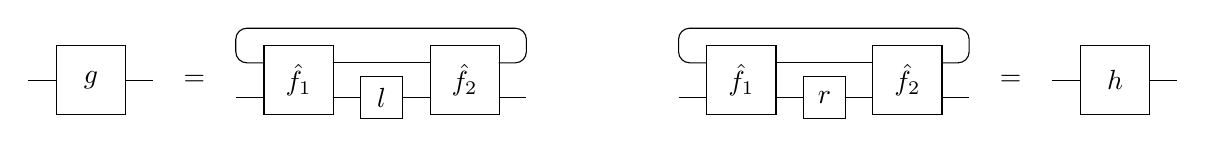
\begin{tikzpicture}[yscale=-1,x=1em,y=1.25em]

    \draw (0,3) -- (1,3);
    \node [draw, minimum width=2.5em, minimum height=2.5em, anchor=west] at (1,3) {$g$};
    \draw (3.5,3) -- (4.5,3);

    \node at (6,3) {$=$};

    \draw (7.5,3.5) -- (8.5,3.5);
    \node [draw, minimum width=2.5em, minimum height=2.5em, anchor=west] at (8.5,3) {$\hat{f_1}$};
    \draw (11,2.5) -- (14.5,2.5);
    \draw (11,3.5) -- (12,3.5);
    \node [draw, minimum width=1.5em, minimum height=1.5em, anchor=west] at (12,3.5) {$l$};
    \draw (13.5,3.5) -- (14.5,3.5);
    \node [draw, minimum width=2.5em, minimum height=2.5em, anchor=west] at (14.5,3) {$\hat{f_2}$};
    \draw (17,3.5) -- (18,3.5);
    \draw [rounded corners] (17,2.5) -- (18,2.5) -- (18,1.5) -- (7.5,1.5) -- (7.5,2.5) -- (8.5,2.5);

    \node at (21,3) {$\rewrite_{\mcr}$};

    \draw (23.5,3.5) -- (24.5,3.5);
    \node [draw, minimum width=2.5em, minimum height=2.5em, anchor=west] at (24.5,3) {$\hat{f_1}$};
    \draw (27,2.5) -- (30.5,2.5);
    \draw (27,3.5) -- (28,3.5);
    \node [draw, minimum width=1.5em, minimum height=1.5em, anchor=west] at (28,3.5) {$r$};
    \draw (29.5,3.5) -- (30.5,3.5);
    \node [draw, minimum width=2.5em, minimum height=2.5em, anchor=west] at (30.5,3) {$\hat{f_2}$};
    \draw (33,3.5) -- (34,3.5);
    \draw [rounded corners] (33,2.5) -- (34,2.5) -- (34,1.5) -- (23.5, 1.5) -- (23.5,2.5) -- (24.5,2.5);

    \node at (35.5,3) {$=$};

    \draw (37,3) -- (38,3);
    \node [draw, minimum width=2.5em, minimum height=2.5em, anchor=west] at (38,3) {$h$};
    \draw (40.5,3) -- (41.5,3);

\end{tikzpicture}
\end{document}
